\section{Theorie}
\label{sec:Theorie}

\subsection{Gedämpfte Schwingungen}
\label{sec:gedschw}

Ein gedämpfter elektrischer Schwingkreis ist beispielsweise ein \textbf{RCL}-Kreis.
In Abbildung \ref{fig:rcl} ist einer abgebildet.
Dort schwingt die elektrische Energie zwischen dem Kondensator und der Spule
hin und her. Doch am Widerstand wird ein Teil der Energie in Wärmeenergie umgewandelt.
So wird dem System Energie entzogen und die Schwingungsamplitude nimmt ab.

\begin{figure}[h]
  \centering
  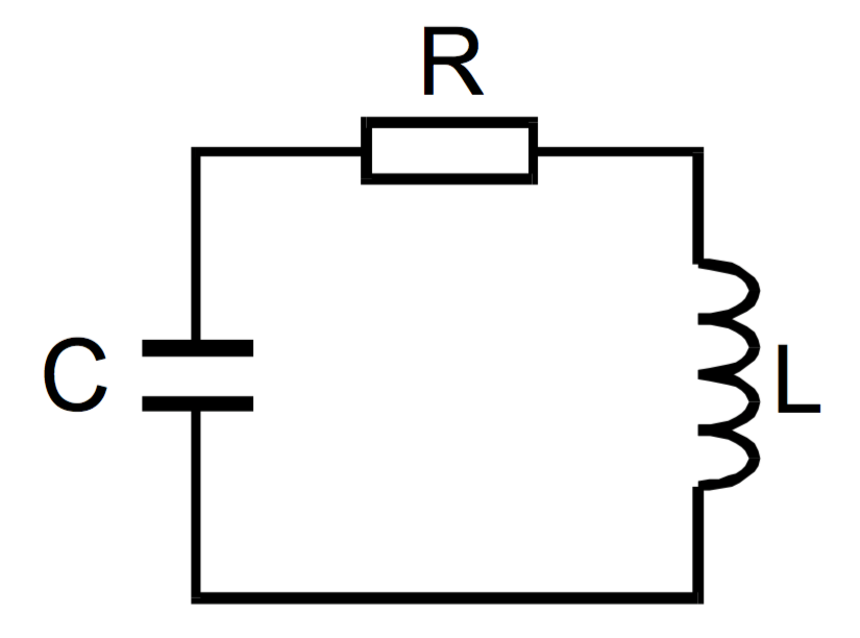
\includegraphics[height = 3 cm]{RCL.pdf}
  \caption{Eine \textbf{RCL}-Schaltung \cite{anleitung}.}
  \label{fig:rcl}
\end{figure}

Über das 2.Kirchhoffsche Gesetz, dass die Summe aller Spannungen null ist, ergibt
sich folgende Differentialgleichung:

\begin{equation}
  \frac{\symup{d}^2 \g{I}}{\symup{d t}^2} + \frac{\symup{R}}{\symup{L}}
  \frac{\g{d I}}{\g{d t}} + \frac{1}{\g{L C}} \g{I} = 0.
  \label{eqn:dgl}
\end{equation}

Als Lösungen ergeben sich die folgenden:

\begin{equation}
  \mathfrak{I}(t) = \mathfrak{U}_1 \textbf{e}^{\g{i\tilde{\omega}_1t}} + \mathfrak{U}_2
  \textbf{e}^{\g{i\tilde{\omega}_2t}}.
\end{equation}

$\mathfrak{U}_1$ und $\mathfrak{U}_2$ sind hierbei beliebige komplexe Zahlen.
$\g{\tilde{\omega}}_\text{1}$ und $\g{\tilde{\omega}}_\text{1}$ sind Konstanten nach Gleichung
\eqref{eqn:konstant}.

\begin{equation}
  \tilde{\omega}_{1,2} = \g{i\frac{R}{2 L} \pm \sqrt{\frac{1}{L C} - \frac{R^2}{4 L^2}}}
  \label{eqn:konstant}
\end{equation}

Mit den Abkürzungen

\begin{align}
  2 \pi \mu := \g{\frac{R}{2 L}} \quad \text{und} \quad 2 \pi \g{\tilde{\nu}} := \g{\sqrt{\frac{1}{L C} - \frac{R^2}{4 L^2}}}
  \label{eqn:abk}
\end{align}

ergibt sich, bei reellem $\tilde{\nu}$ in Gleichung \eqref{eqn:abk}, die Gleichung \eqref{eqn:gedschw}.

\begin{equation}
  I(t) = A_0 \g{e}^{-2 \g{\pi} \mu t} \cos(2 \g{\pi} \nu t + \eta)
  \label{eqn:gedschw}
\end{equation}

Klar zu erkennen ist hier die Oszillation und die exponentielle Abnahme.
In Abbildung \ref{fig:gedschw} ist dies auch zu erkennen.

\begin{figure}[h]
  \centering
  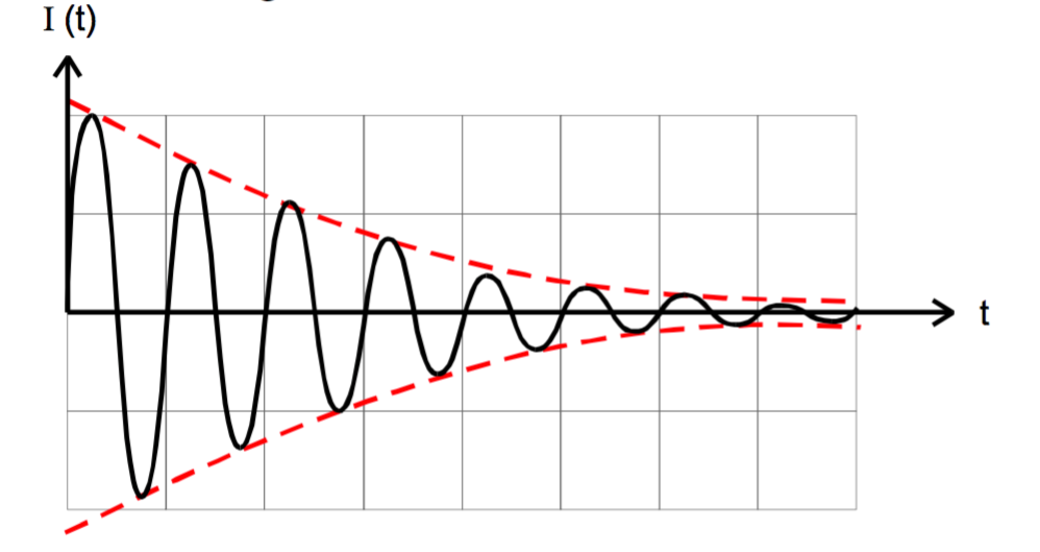
\includegraphics[height = 5cm]{gedschw.pdf}
  \caption{Eine gedämpfte Schwingung mit der Einhüllenden $\pm e^{-2\g{\pi}\mu t}$ \cite{anleitung}.}
  \label{fig:gedschw}
\end{figure}

Die Schwingungsdauer nähert sich dabei nach Gleichung \eqref{eqn:Tschwing}.

\begin{equation}
  T_{\text{0}} = \frac{2 \pi}{\omega_0} = 2 \g{\pi}\sqrt{\g{LC}}
  \label{eqn:Tschwing}
\end{equation}

Die Abklingdauer, nach der die Amplitude auf den e-ten Teil abgefallen ist,
berechnet sich nach Gleichung \eqref{eqn:Tex}.

\begin{equation}
  T_{\text{ex}} = \frac{1}{2\g{\pi}\mu} = \frac{2\g{L}}{\g{R}}
  \label{eqn:Tex}
\end{equation}

\subsection{Aperiodischer Grenzfall}

Nun wird der Fall betrachtet, der auftritt wenn gilt:
$1/LC = R_{ap}^2/4L^2$. Dann wird nämlich $\nu = 0$ und die Lösung stellt
sich wie in Gleichung \eqref{eqn:aperio} dar:

\begin{equation}
  I(t) = A \g{e}^{-\frac{R}{2L}\cdot t} = A \g{e}^{-\frac{t}{\sqrt{LC}}}.
  \label{eqn:aperio}
\end{equation}

\begin{figure}[h]
  \centering
  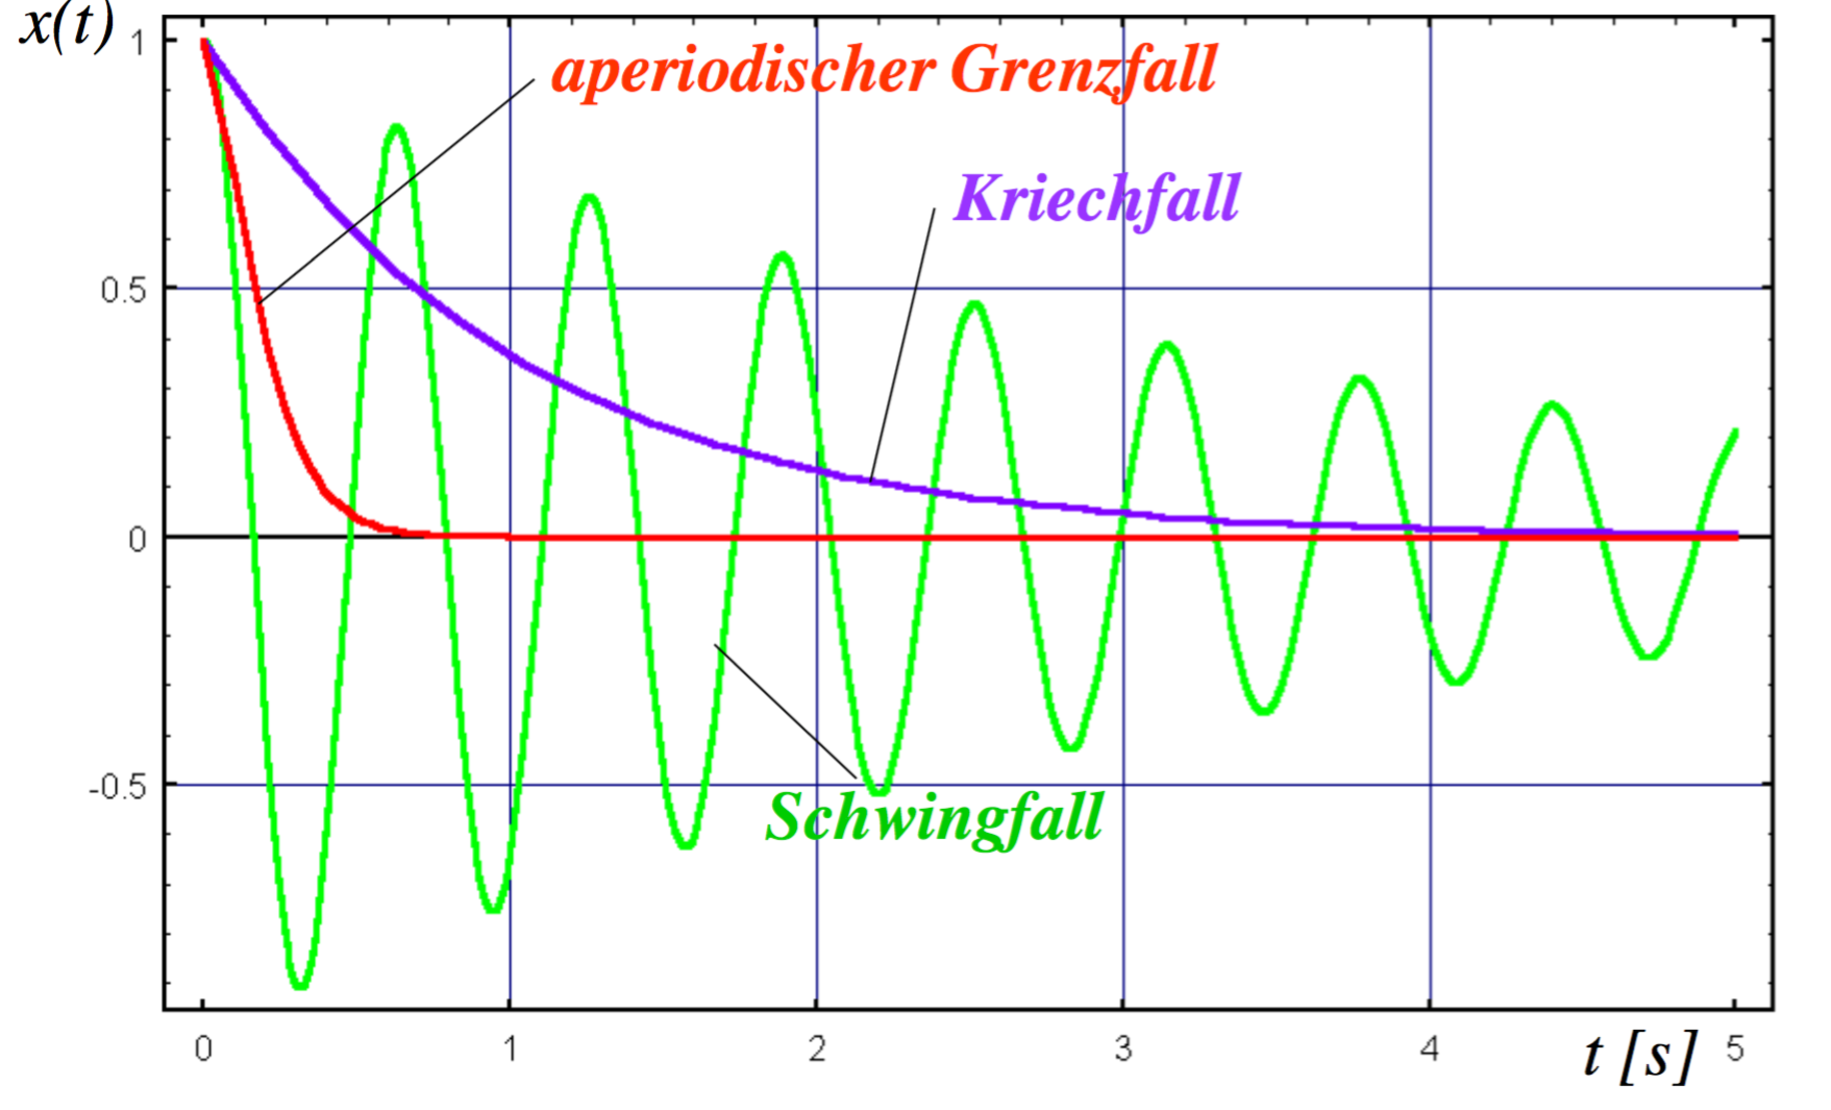
\includegraphics[height = 8cm]{aperio.pdf}
  \caption{Schwingungsformen bei gedämpftem Schwingkreis mit $x(t) = I(t)$ \cite{weis}.}
  \label{fig:aperio}
\end{figure}

In Abbildung \ref{fig:aperio} ist der aperiodische Grenzfall, der
Schwingfall, der in Kapitel \ref{sec:gedschw} thematisiert wird, und
außerdem der Kriechfall zu sehen.

\subsection{Erzwungene Schwingungen}

\begin{figure}[h]
  \centering
  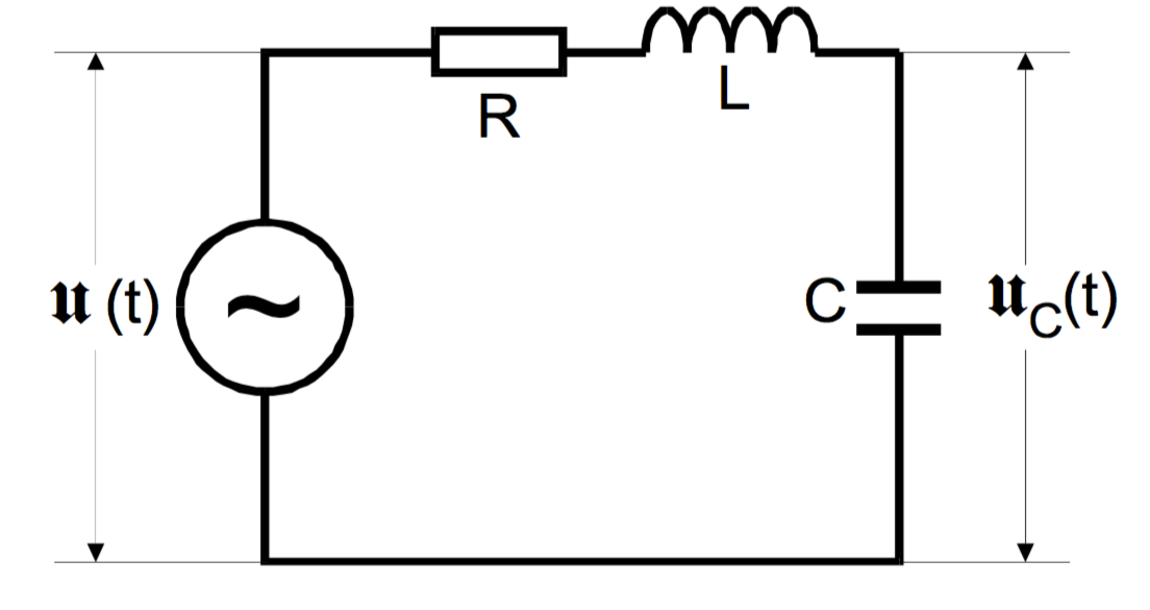
\includegraphics[height = 5cm]{erzwschw.pdf}
  \caption{Schaltkreis zur Erzeugung einer erzwungenen Schwingung innerhalb
  eines elektrischen Schwingkreises \cite{anleitung}.}
  \label{fig:erzwschw}
\end{figure}

In Abbildung \ref{fig:erzwschw} ist ein neuer Schaltkreis abgebildet. Hier
wird nun durch einen Sinus-Generator eine Wechselspannung  $\mathfrak{U}(t)$
an das System angelegt.

Über die Differentialgleichung \eqref{eqn:dglerzw}

\begin{equation}
  L\frac{\g{d}\mathfrak{I}}{\g{dt}} + R\mathfrak{I} + \frac{\mathfrak{C}}{\g{C}}
   = U_{\text{0}}\g{e}^{i\omega t}
  \label{eqn:dglerzw}
\end{equation}
ergibt sich für die Kondensatorspannung $U_C$ in Abhängigkeit von der
Kreisfrequenz $\omega$ die Gleichung \eqref{eqn:ukonden}.

\begin{equation}
  U_C(\omega) = \frac{U_\text{0}}{\sqrt{(1 - LC\omega^2)^2 + \omega^2
  R^2C^2}}
  \label{eqn:ukonden}
\end{equation}

Dabei ist $\omega = 2 \g{\pi} \nu$. Der Verlauf dieser Kurve stellt sich
so dar, dass die Kurve für $\omega \to \infty$ gegen 0 geht und für
$\omega \to 0$ gegen den Wert der Erregeramplitude $U_0$ strebt.
Zwischen diesen beiden Werten besitzt die Kurve ein Extremum, das
größer als $U_0$ sein kann. Die Frequenz, bei der das der Fall ist,
heißt $\omega_{\text{res}}$; berechnet wird sie folgt:

\begin{equation}
  \omega_{\text{res}} = \sqrt{\frac{1}{LC} - \frac{R^2}{2L^2}}.
\end{equation}

Wenn das System nur schwach gedämpft ist, $\frac{R^2}{2L^2}$ also viel
kleiner ist als $\frac{1}{LC}$, nähert sich $\omega_{\text{res}}$ der
Kreisfrequenz $\omega{\text{0}}$ der ungedämpften Schwingung an.

Dann übertrifft $U_C$ die Erregerspannung $U_0$ um den Faktor $q$ nach
Gleichung \eqref{eqn:resoueber} mit

\begin{equation}
  q = \frac{1}{\omega_0RC} = \frac{1}{R}\sqrt{\frac{L}{C}}.
\end{equation}

\begin{equation}
  U_{C,max} = q U_{\text{0}}
  \label{eqn:resoueber}
\end{equation}

$q$ wird als Resonanzüberhöhung oder Güte bezeichnet.
Sie kann auch über die Breite zwischen den beiden Frequenzen $\omega_+$
und $\omega_-$ an denen $U_C$ auf den Bruchteil $1/\sqrt{2}$ des
Maximalwerts abgesunken ist. Dann folgt für die Güte

\begin{equation}
  q = \frac{\omega_{\text{0}}}{\omega_+ - \omega_-}.
\end{equation}
